\chapter{Produto Final}
\label{sec:produto-final}

Esta secção começa com uma pequena apresentação da plataforma desenvolvida (i. e. o estado final da plataforma) e acaba com uma pequena secção onde é descrito os planos futuros para o projecto.


\section{Apresentação da Plataforma}

Nesta secção, será apresentada de forma breve o resultado do desenvolvimento da plataforma de Inbound Marketing. Todas as suas funcionalidades são acedidas através do \textit{browser} e é necessário iniciar sessão. Para efectuar a autenticação é  necessário introduzir o email e password associados à sua conta de utilizador.

Como se pode observar  na Figura \ref{fig:account}, um utilizador pode editar as suas informações pessoais, e caso tenha permissões de adminstração sobre a conta, pode também editar os dados da empresa.

\begin{figure}[ht!]
	\begin{center}
		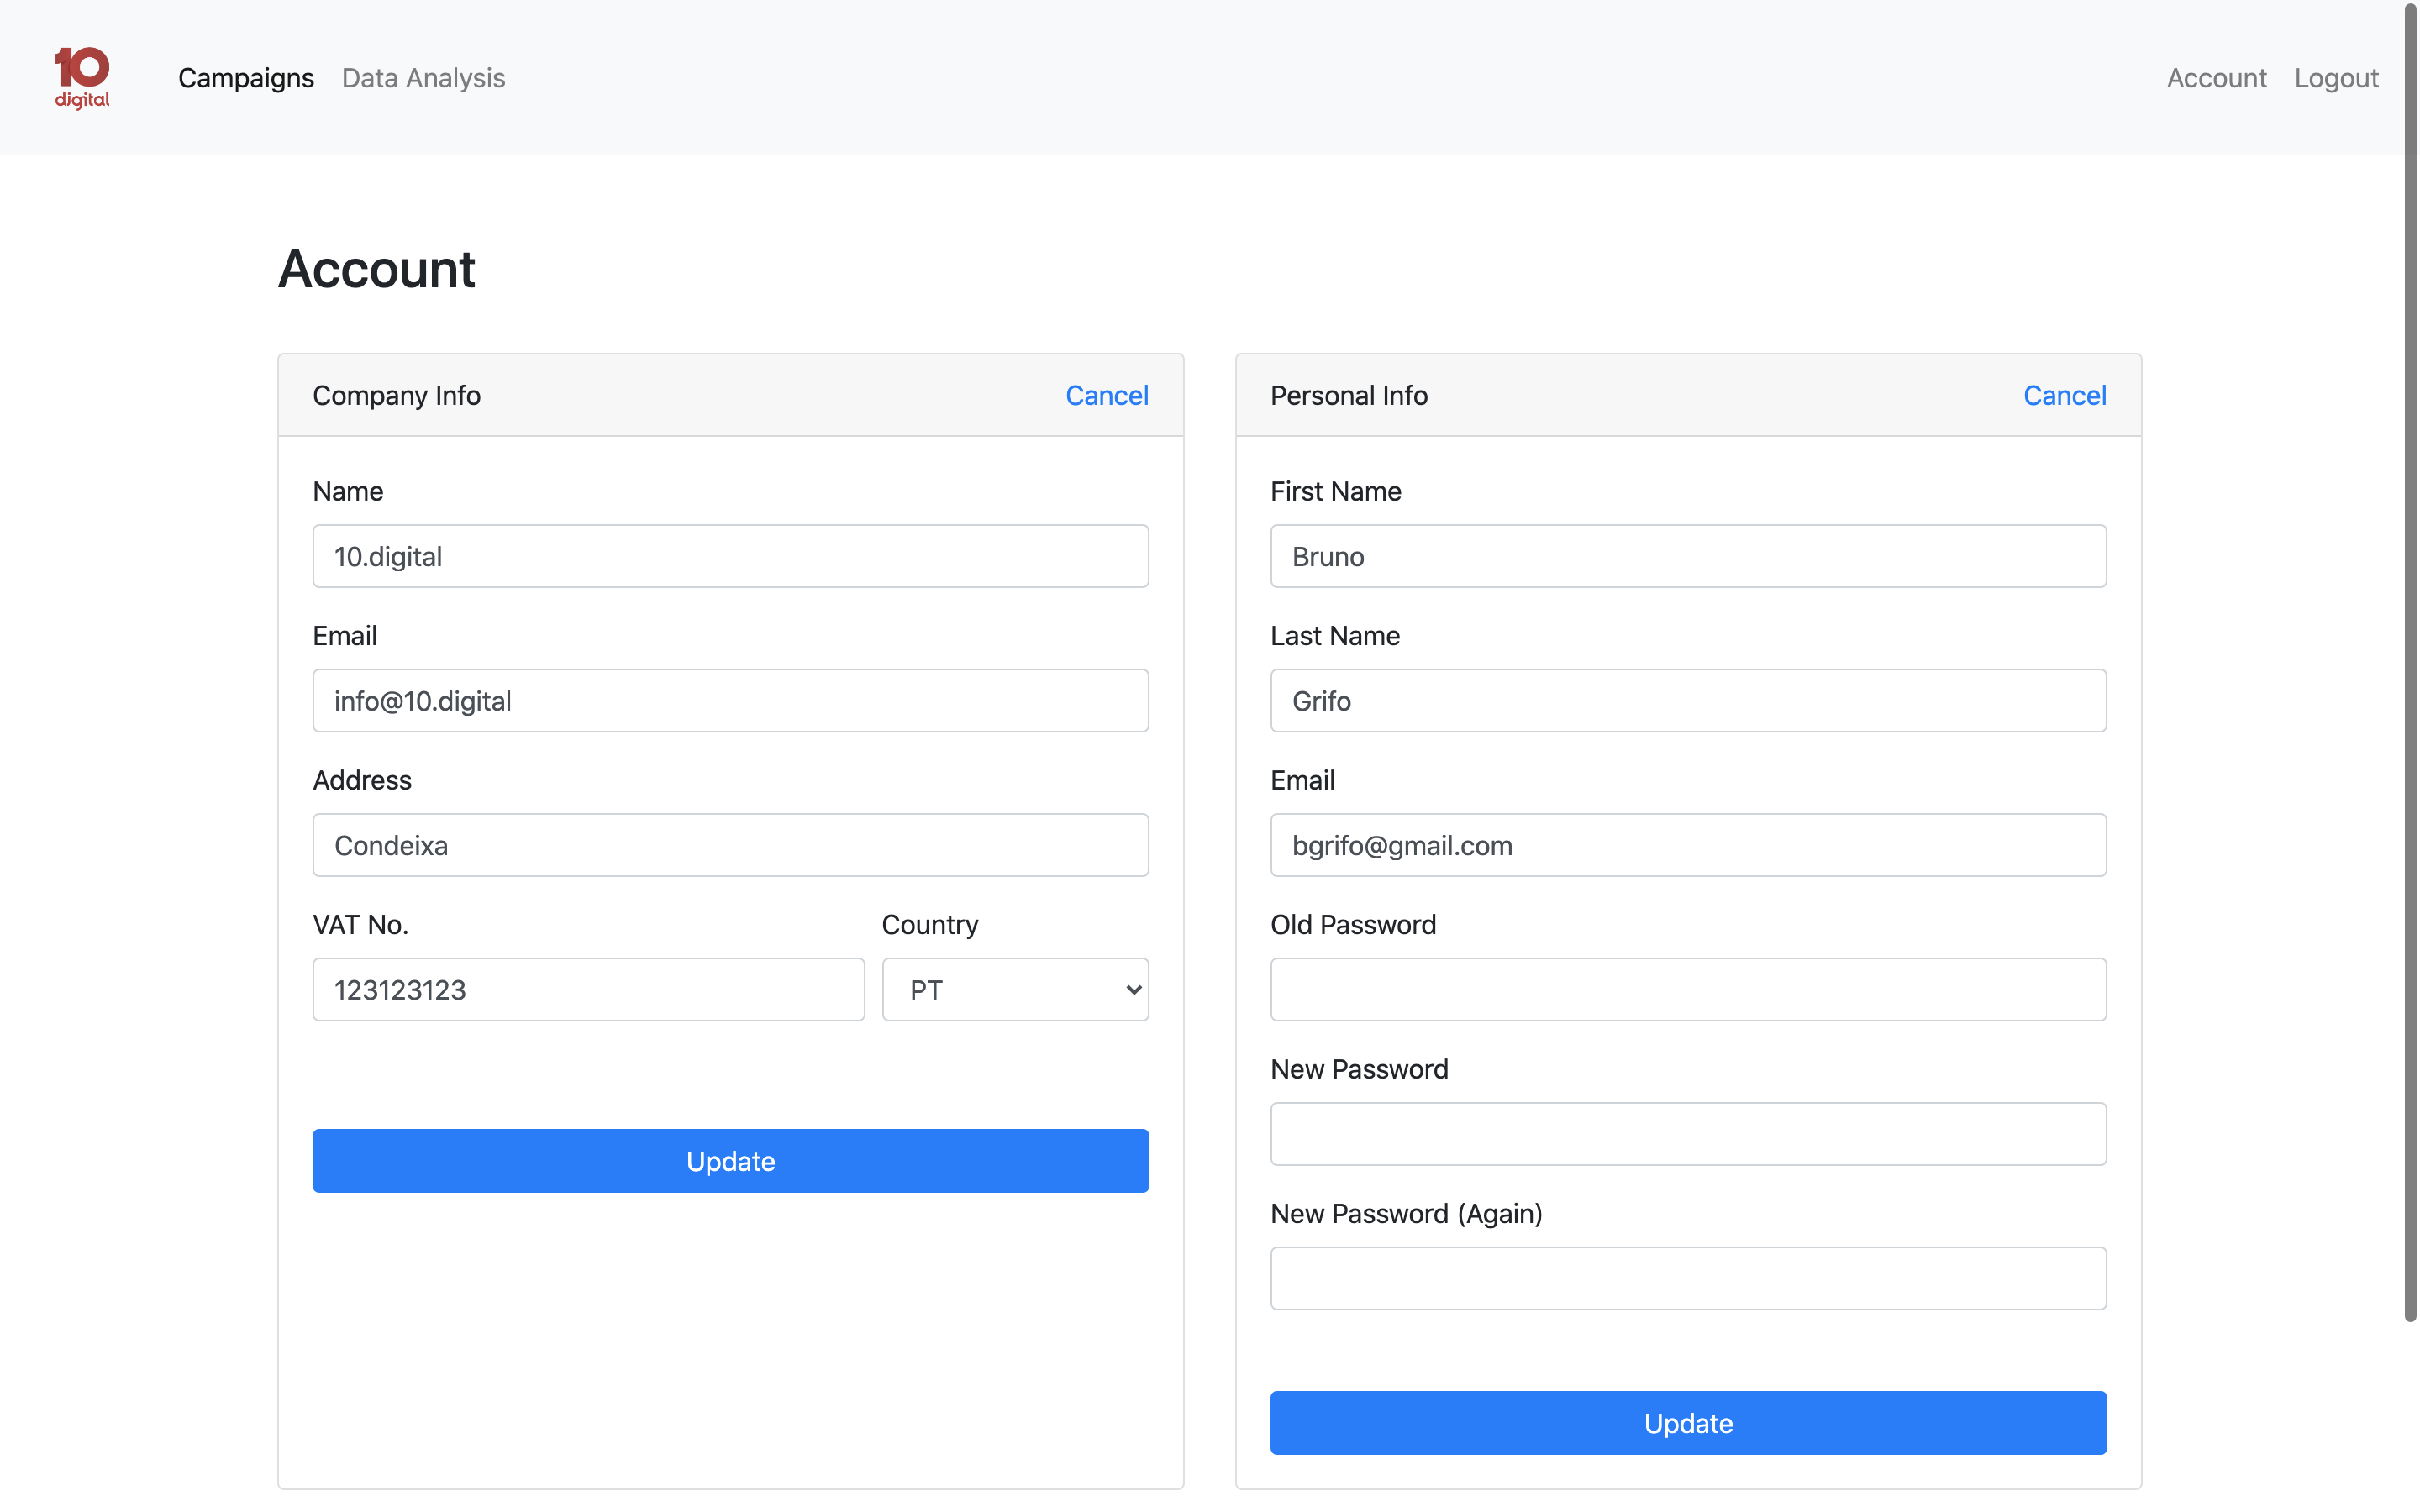
\includegraphics[width=0.8\textwidth]{img/product/account}
		\caption{10.quest - Definições de Conta}
		\label{fig:account}
	\end{center}
\end{figure}

\newpage


Ao entrar na página principal pode-se observar a lista de campanhas, separadas por tipos (i. e. questionários de personalidade e formações), tal como se verifica na Figura \ref{fig:home}. As listas de campanhas mostram também alguns detalhes associados às mesmas como o estado e a data de fim.

Para criar um questionário de personalidade basta carregar no botão que diz "New Personality Quiz" e para editar, basta selecionar um dos questionários de personalidade. Como se pode verificar na Figura \ref{fig:pq} para criar/editar uma campanha do tipo questionário de personalidade, é necessário introduzir um nome, descripção (opcional), data de fim, hora de fim e uma ou mais tags.

\begin{figure}[ht!]
	\begin{center}
		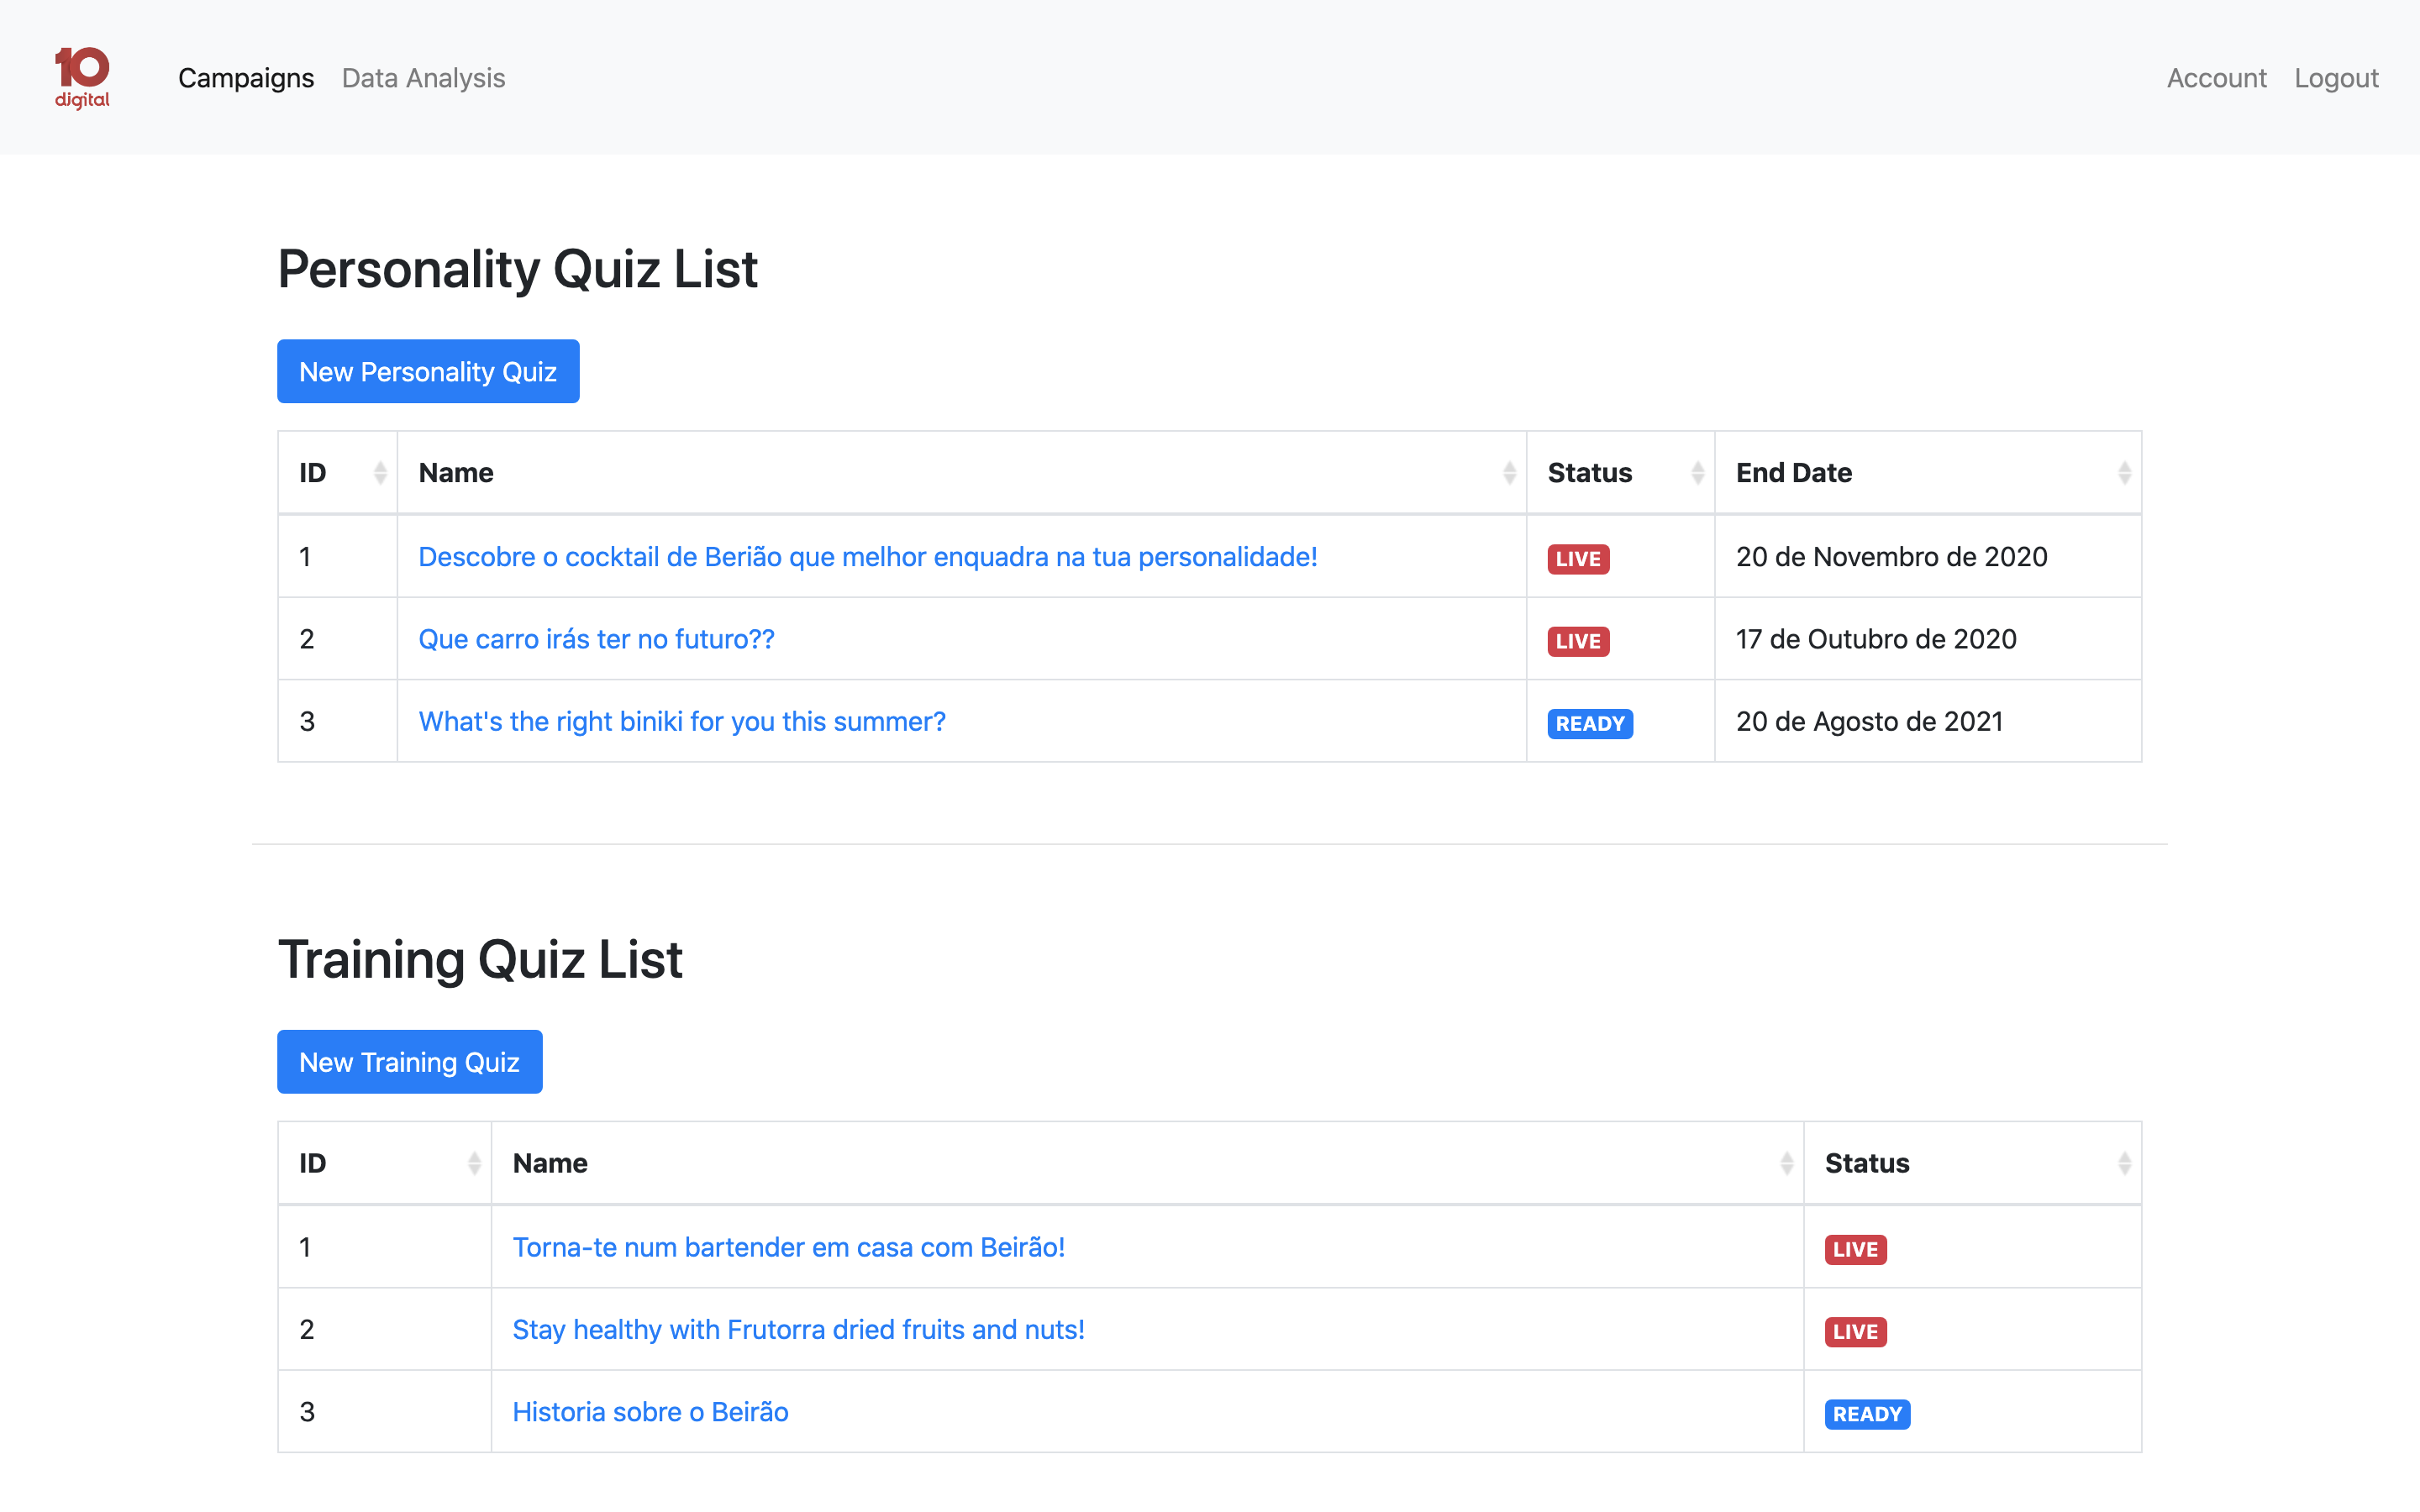
\includegraphics[width=0.8\textwidth]{img/product/homepage}
		\caption{10.quest - Página principal}
		\label{fig:home}
	\end{center}
\end{figure}

\begin{figure}[ht!]
	\begin{center}
		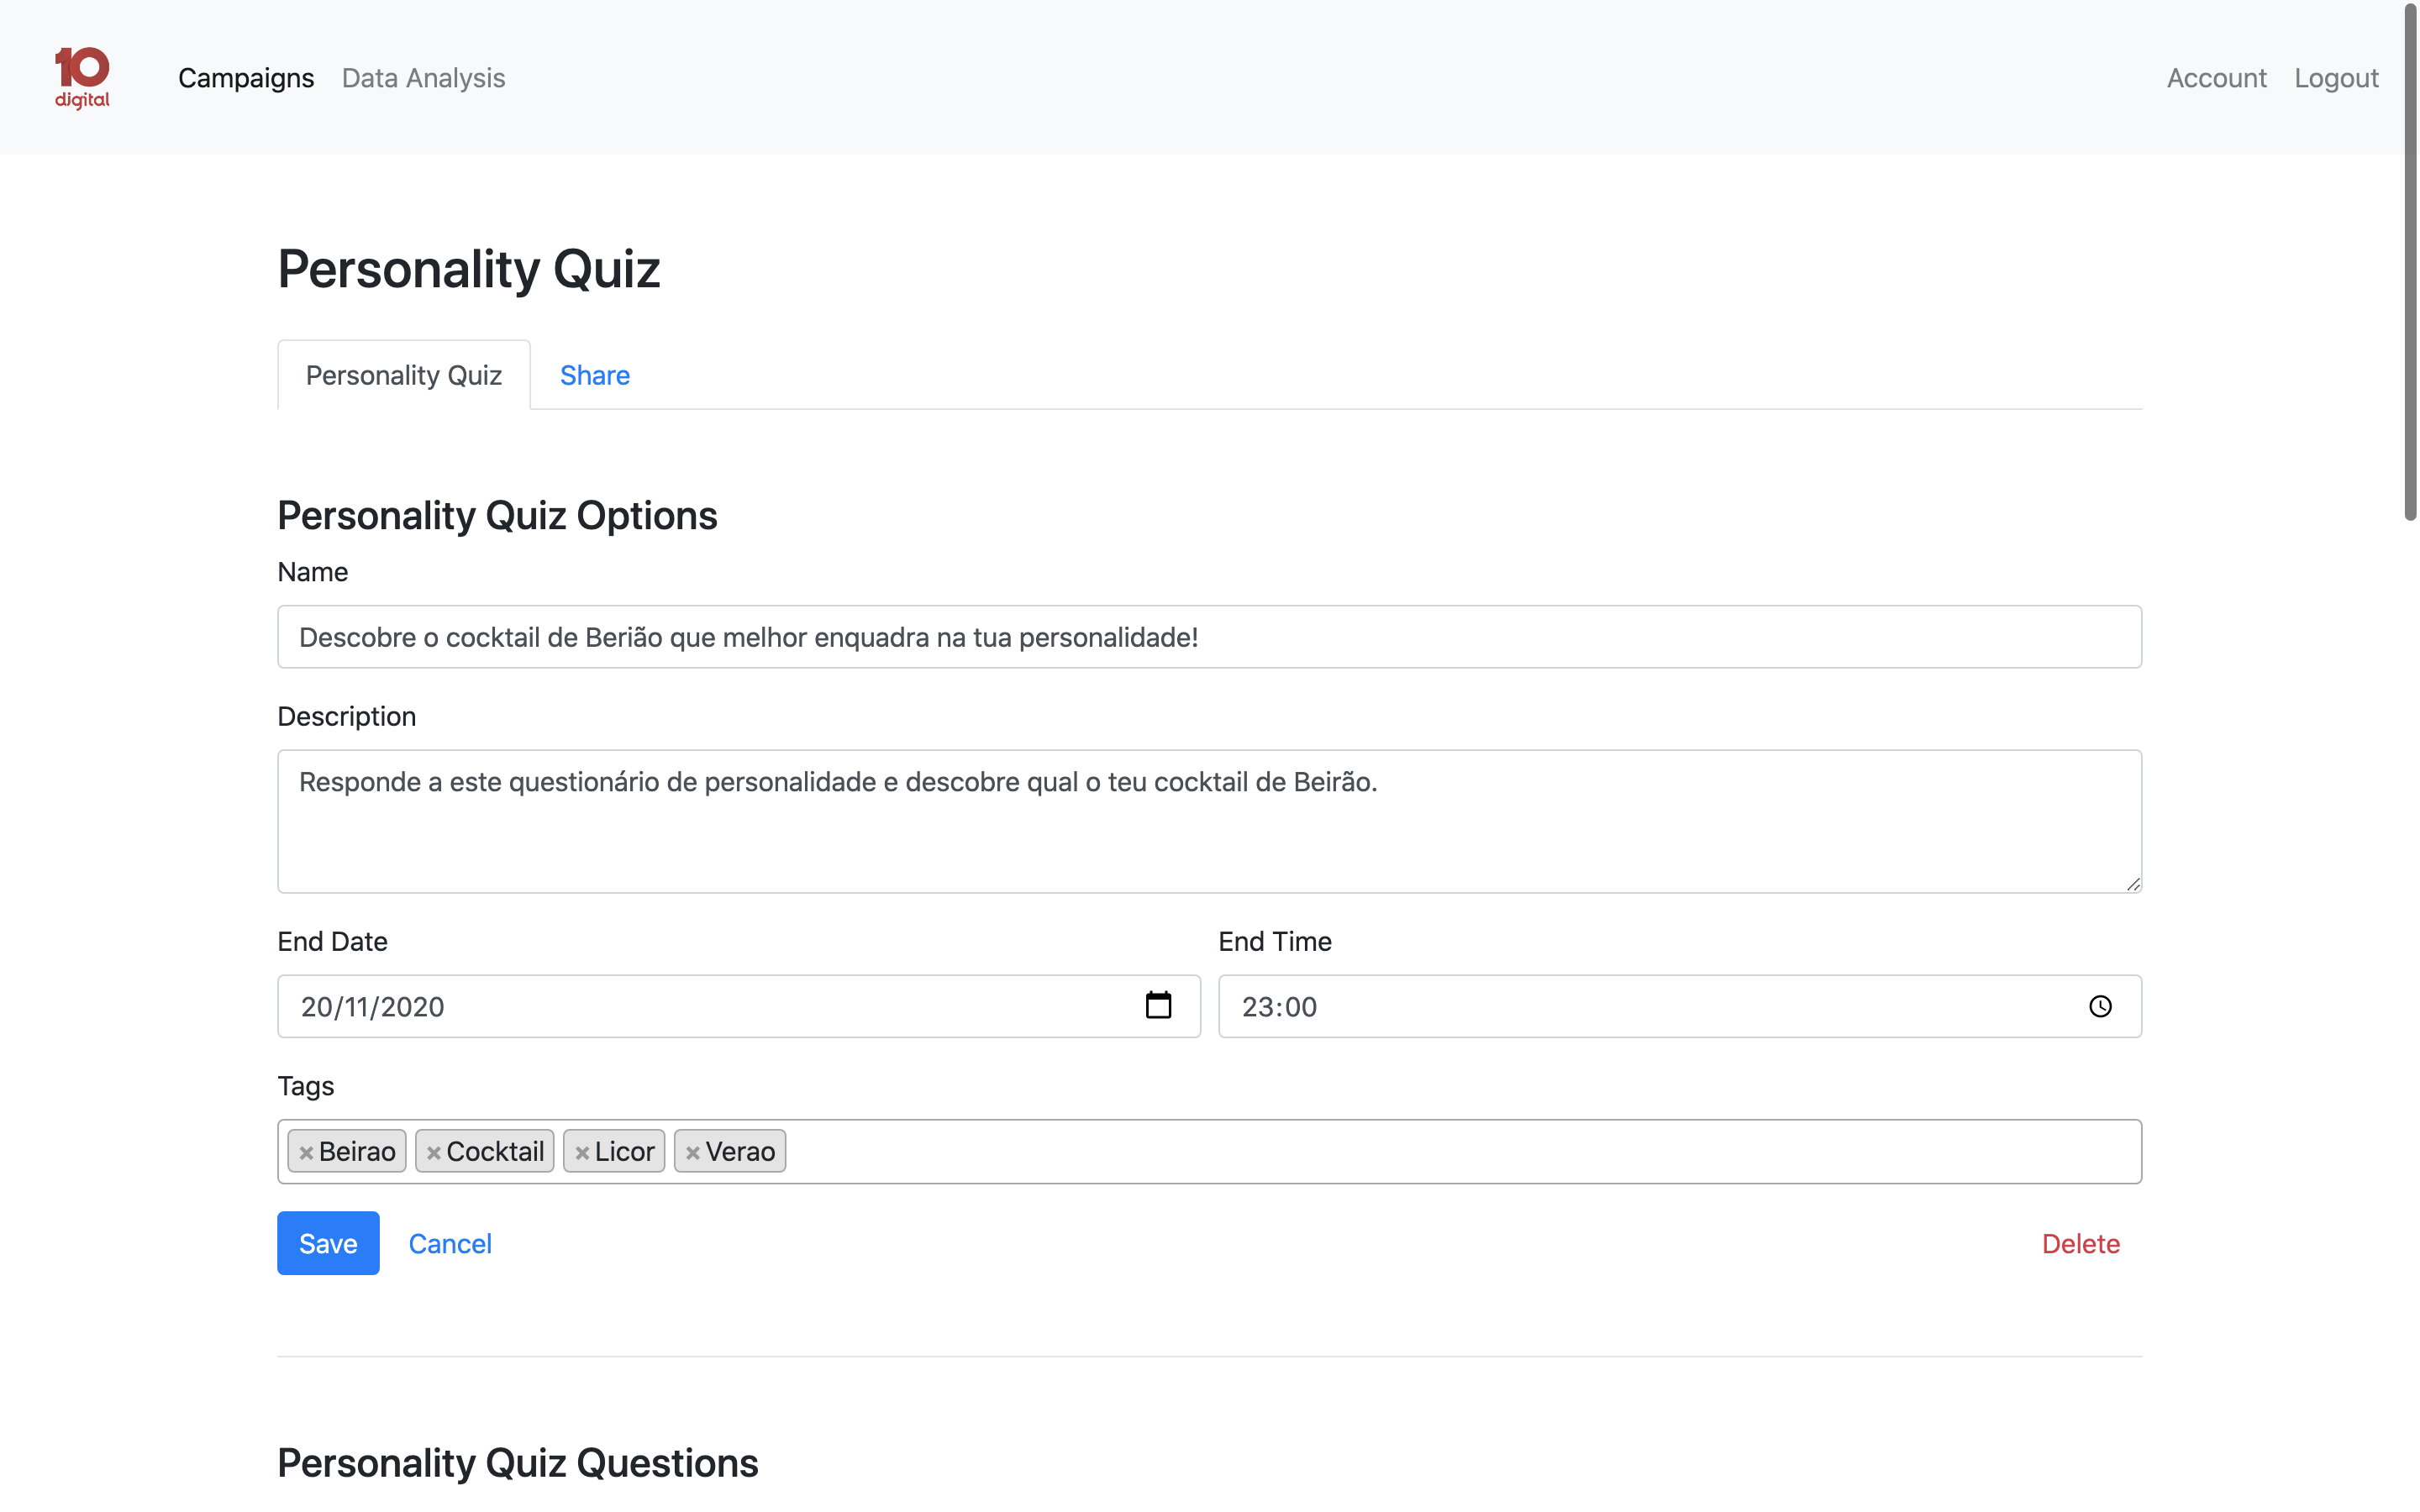
\includegraphics[width=0.8\textwidth]{img/product/pq}
		\caption{10.quest - Criar/Editar Questionário de Personalidade}
		\label{fig:pq}
	\end{center}
\end{figure}
\newpage


Representada na Figura \ref{fig:pq_questions} está a lista de questões associadas ao questionário de personalidade. Para criar uma nova questão é necessário carregar no botão "Create New Question" e para editar basta selecionar uma das questões presentes na lista. É também possível organizar a lista por colunas, pesquisar por nome, importar e exportar questões através de uma \textit{spreadsheet}.

Na criação ou edição de uma questão, como podemos ver na Figura \ref{fig:pq_questions}, é necessário introduzir a pergunta e dar pelo menos duas respostas. O peso atribuido à pergunta está directamente associado com o impacto que a pergunta irá ter no algoritmo de recomendação e os anexos são opcionais.

\begin{figure}[ht!]
	\begin{center}
		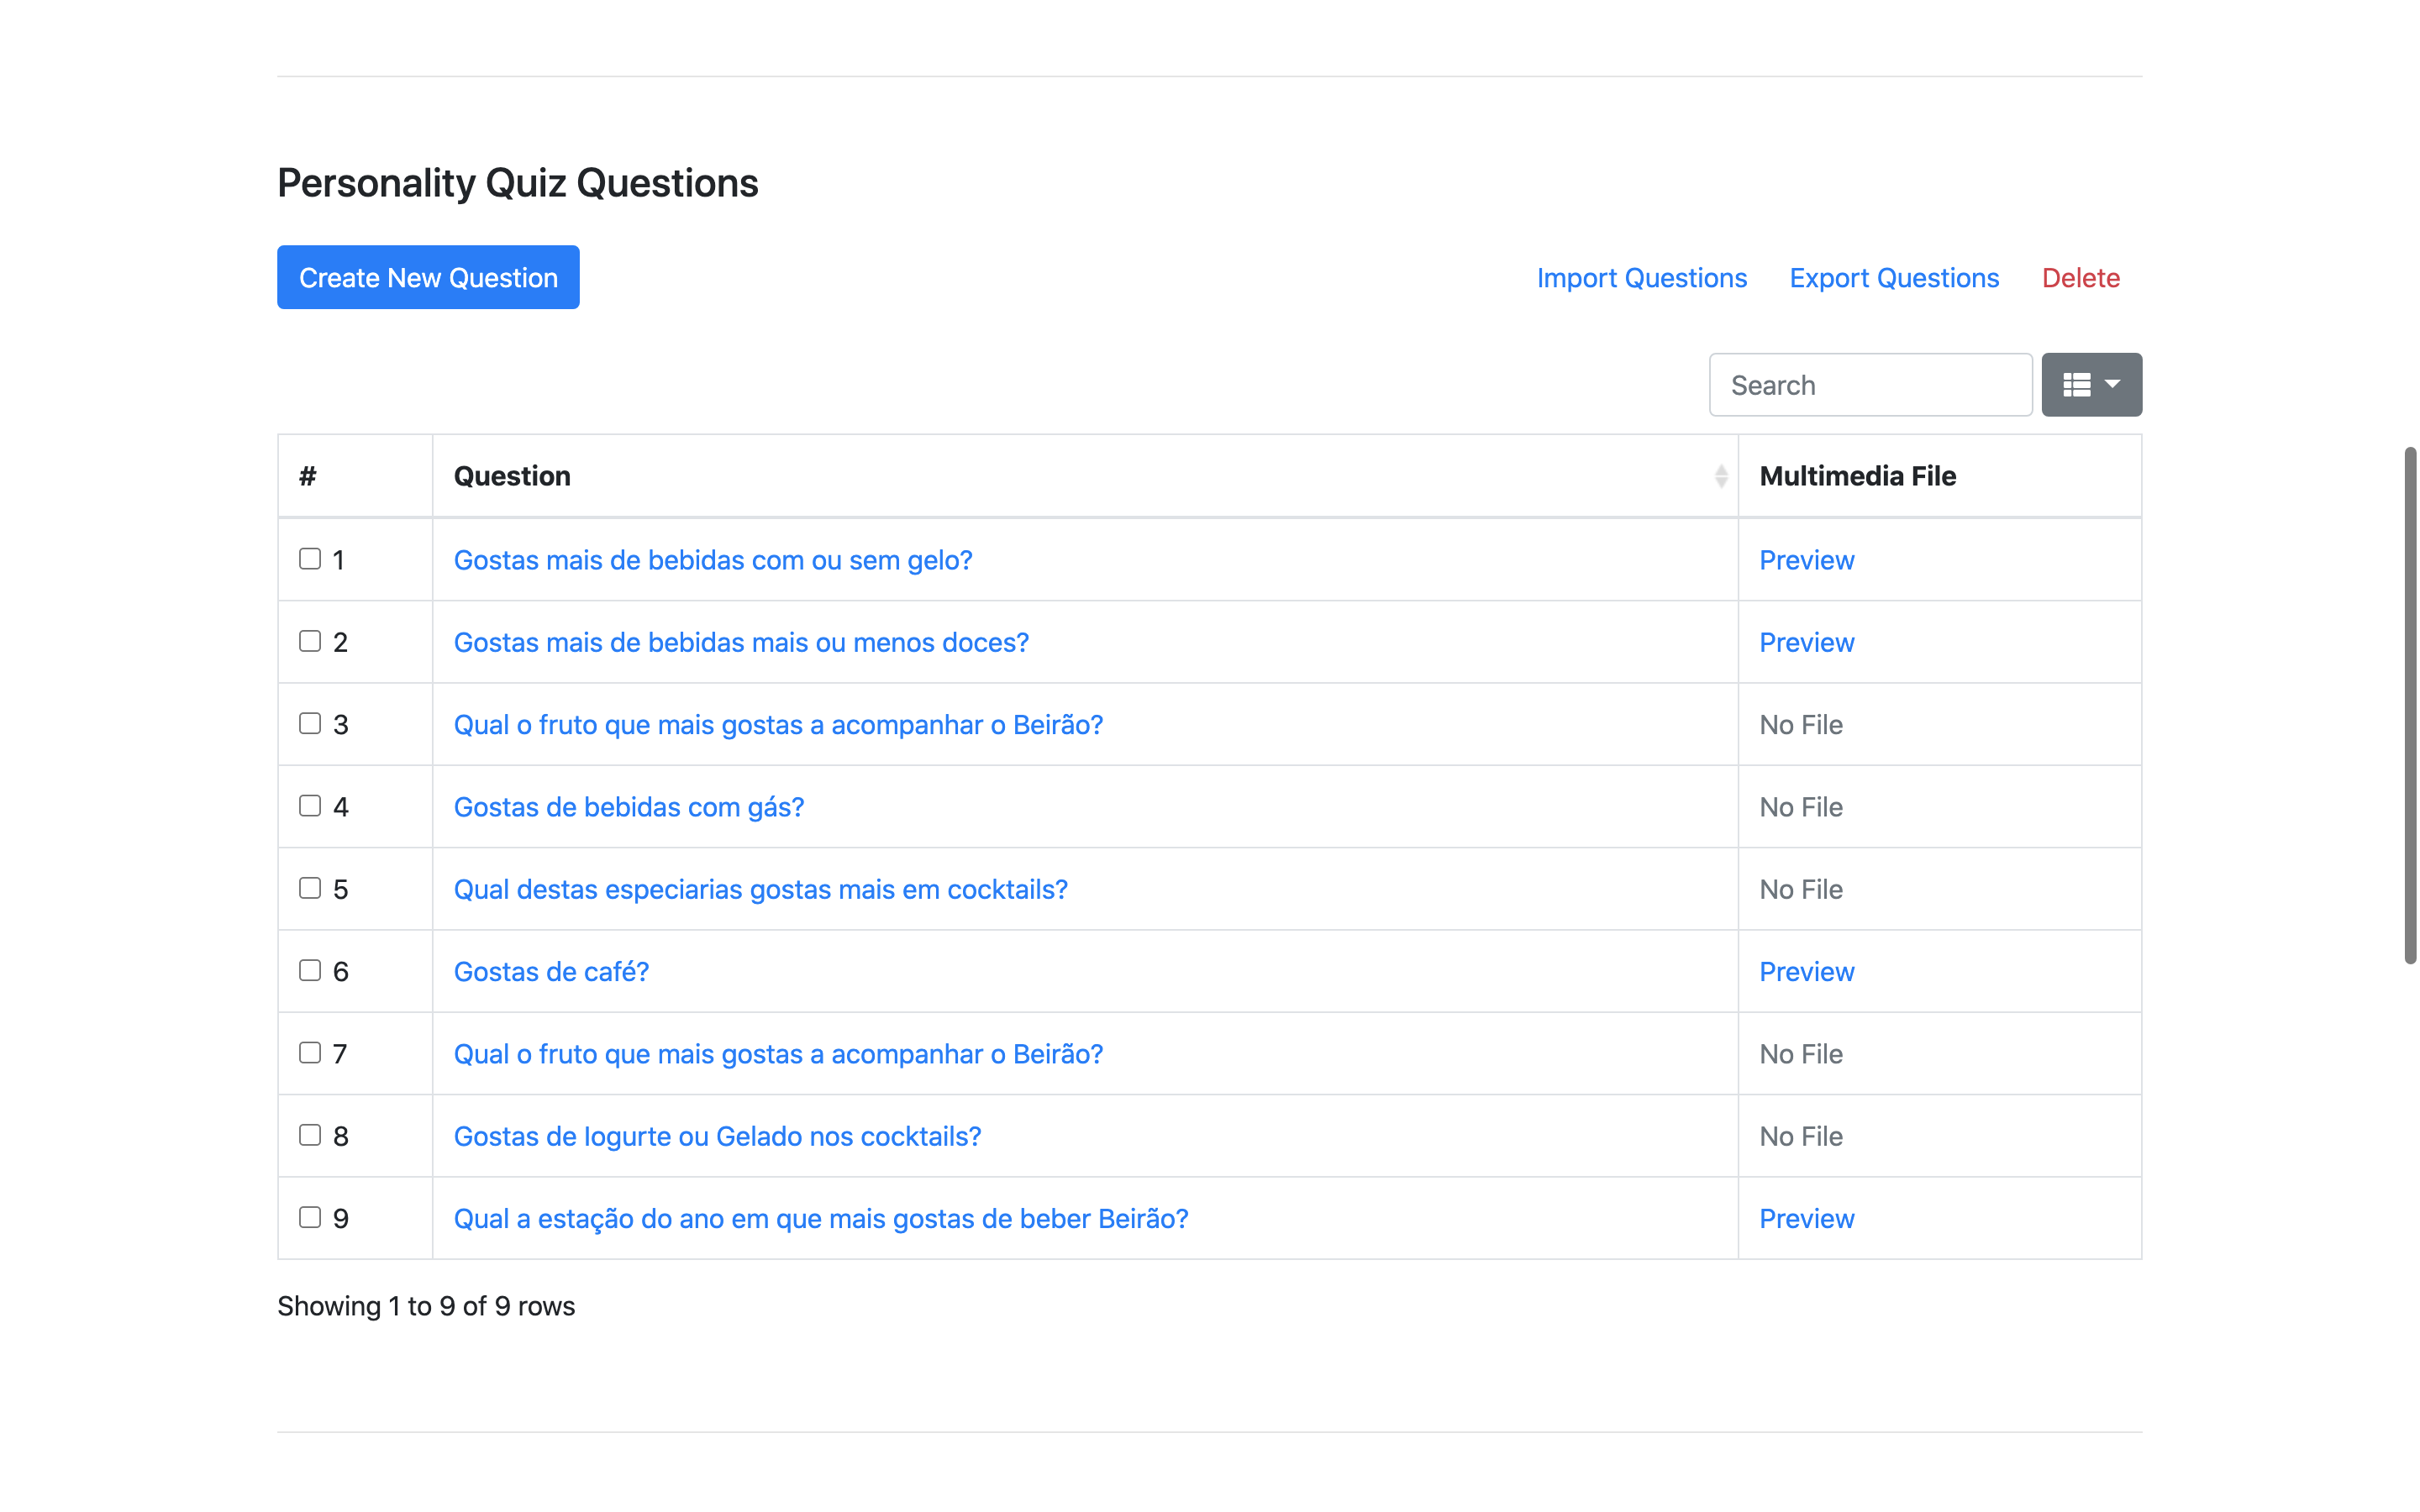
\includegraphics[width=0.8\textwidth]{img/product/pq_questions}
		\caption{10.quest - Lista de questões do Questionário de Personalidade}
		\label{fig:pq_questions}
	\end{center}
\end{figure}


\begin{figure}[ht!]
	\begin{center}
		\begin{minipage}{0.45\textwidth}
			\begin{center}
				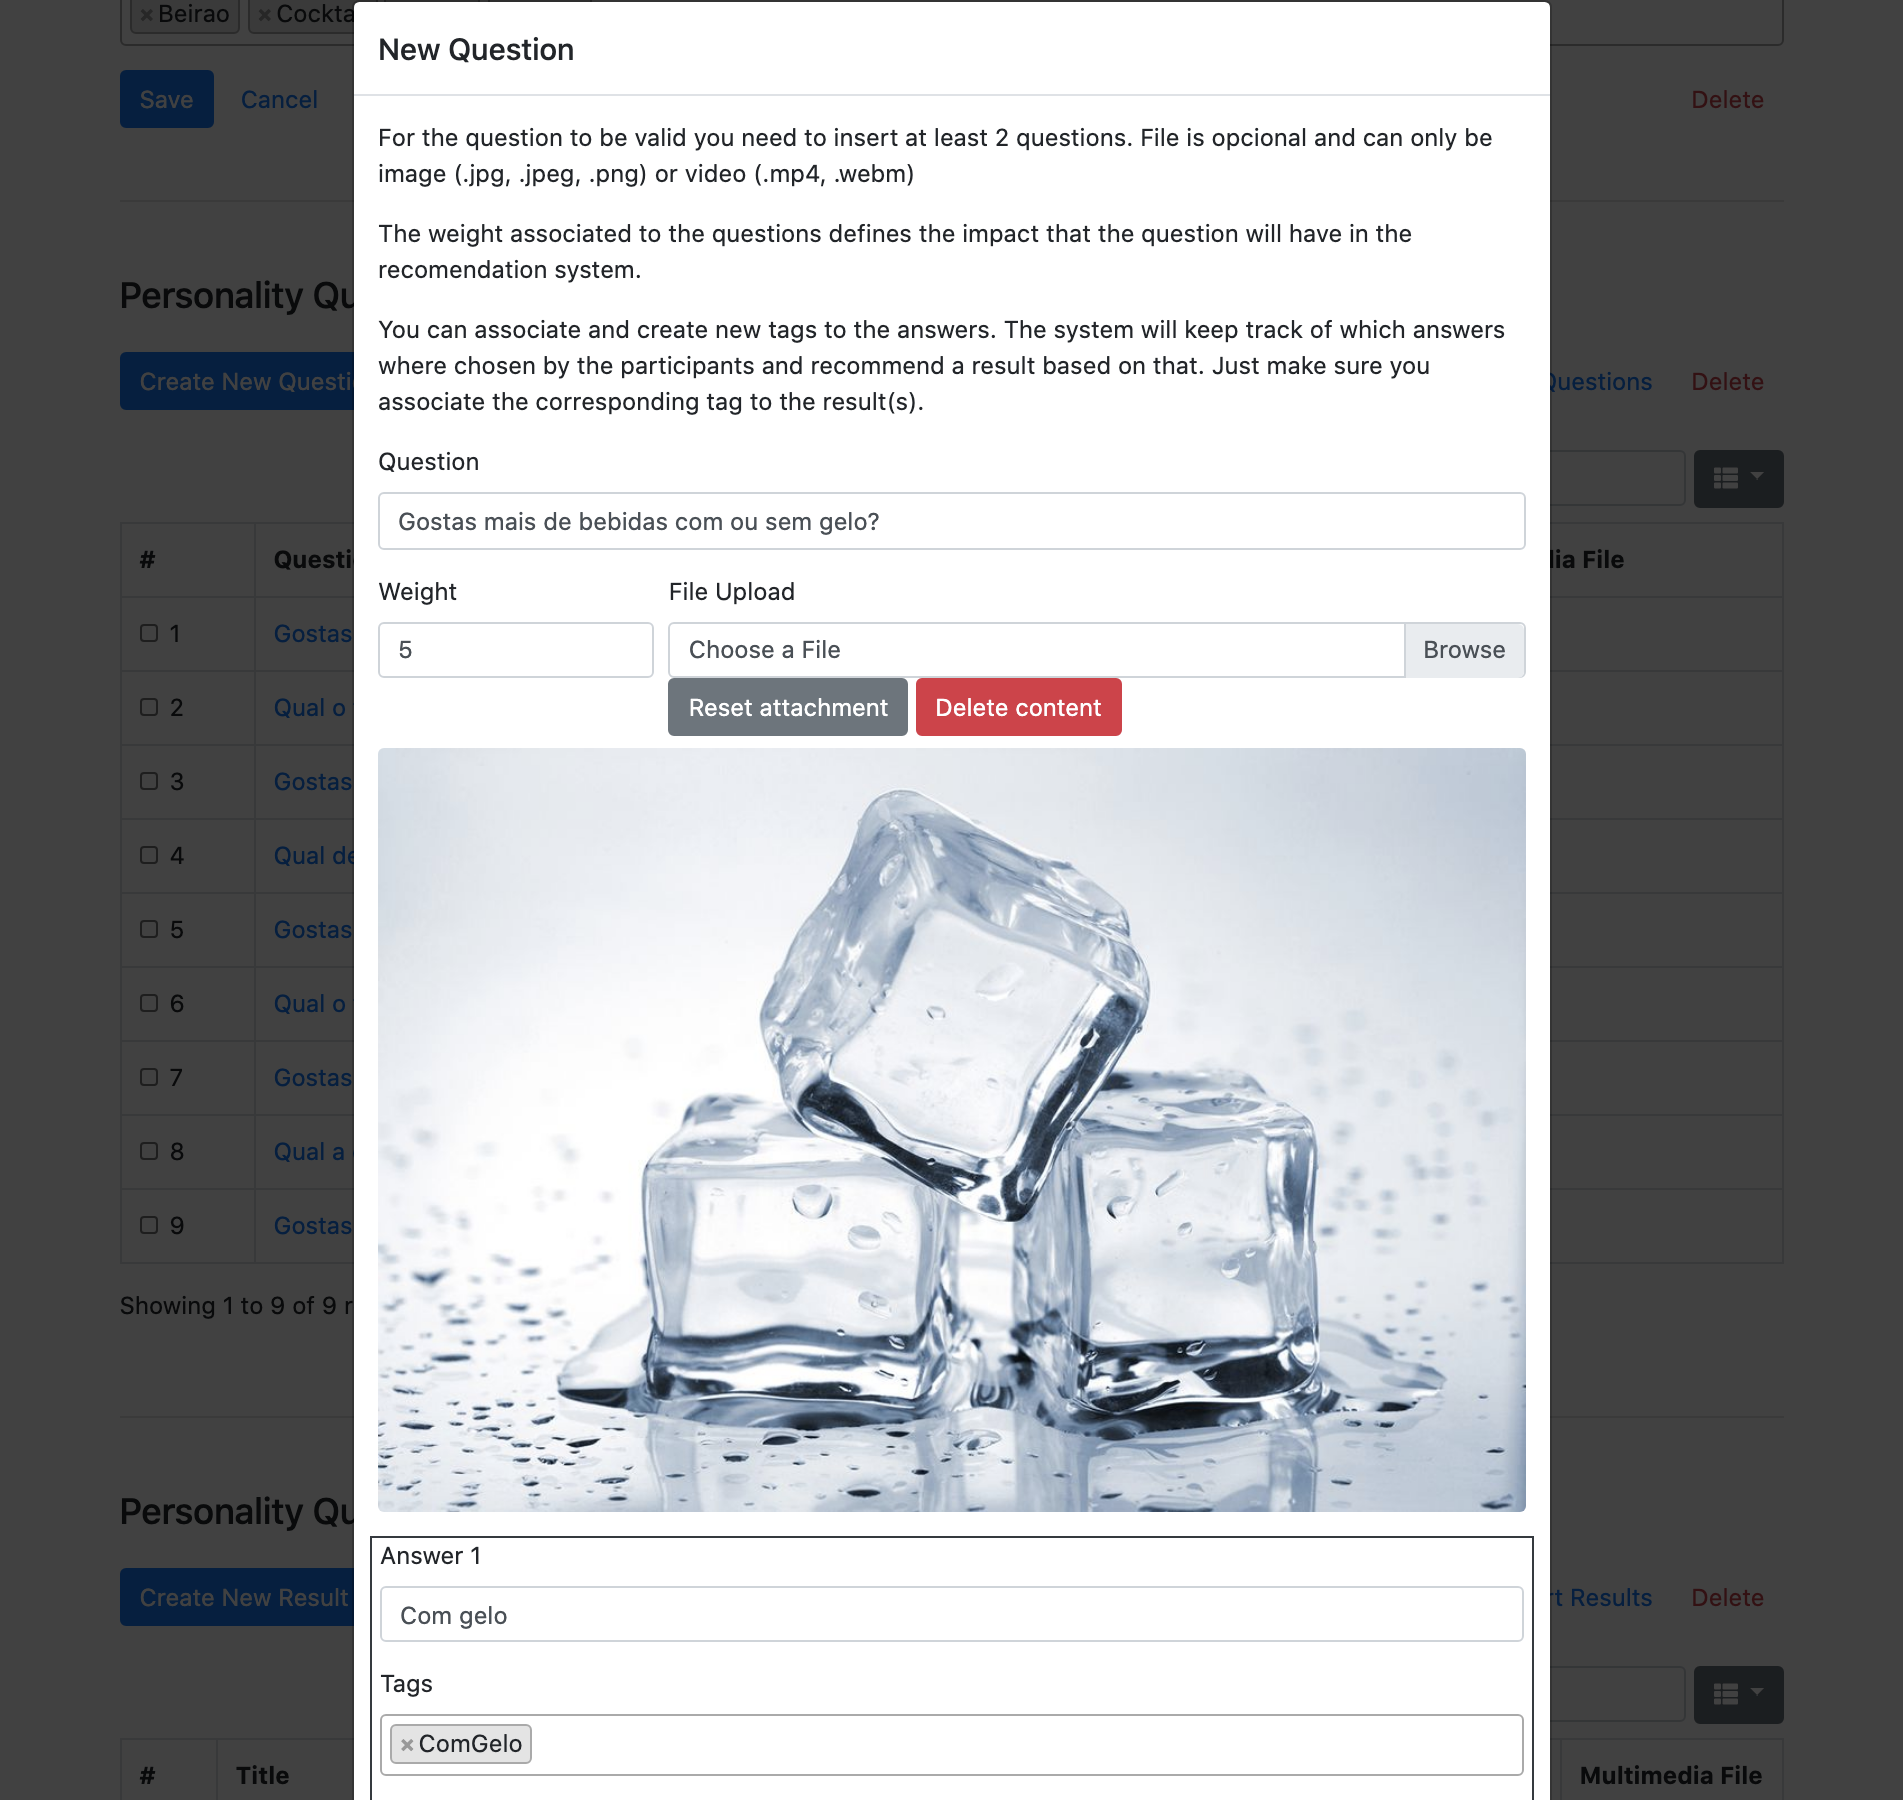
\includegraphics[height=.3\textheight]{img/product/pq_q1}
				\caption{10.quest - Criar/Editar uma questão}
				\label{fig:pq_q1}
			\end{center}
		\end{minipage}
		\hspace{1cm}
		\begin{minipage}{0.45\textwidth}
			\begin{center}
				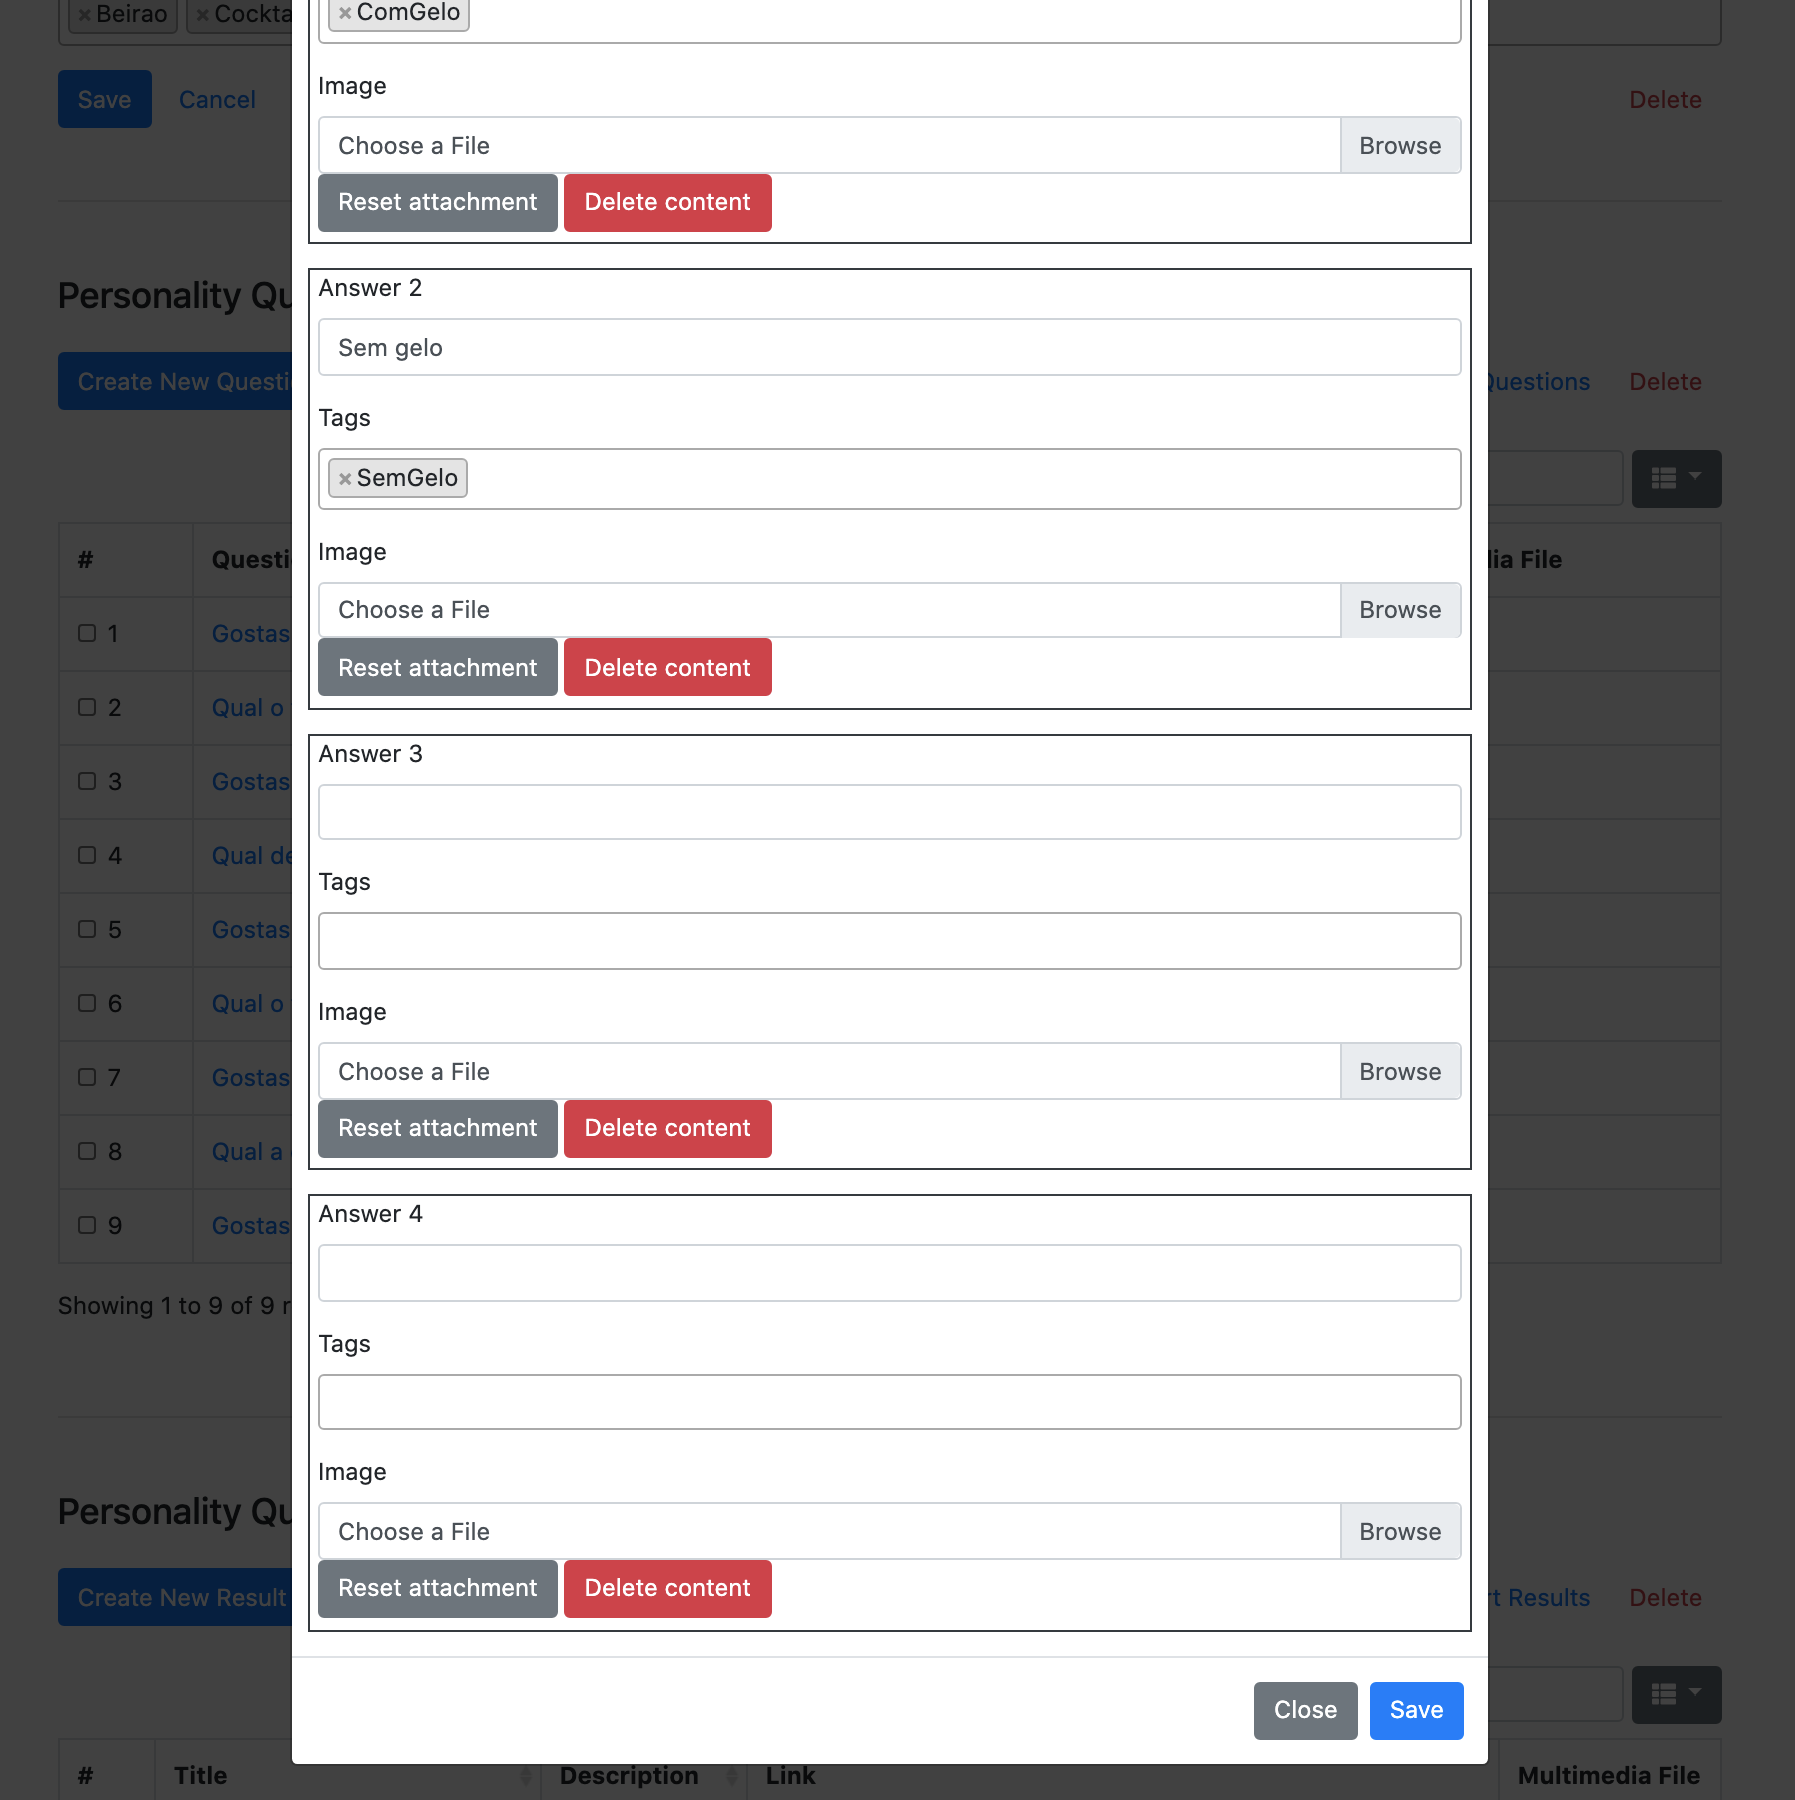
\includegraphics[height=.3\textheight]{img/product/pq_q2}
				\caption{10.quest - Criar/Editar uma questão}
				\label{fig:pq_q2}
			\end{center}
		\end{minipage}
	\end{center}
\end{figure}

\newpage

Representada na Figura \ref{fig:pq_results} está a lista de resultados associados ao questionário de personalidade.Para criar um novo resultado é necessário carregar no botão "Create New Result" e para editar basta selecionar um dos resultados presentes na lista. À semelhança da lista de questões, é também possível organizar a lista por colunas, pesquisar por nome, importar e exportar questões através de uma \textit{spreadsheet}.

Na criação ou edição de um resultado, como podemos ver na Figura \ref{fig:pq_questions}, é necessário introduzir o título e, apesar de não ser obrigatório, é recomendável que sejam associadas uma ou mais tags para que o algoritmo de recomendação devolve algum resultado. Opcionalmente é também possível atribuir uma descrição e um link.

\begin{figure}[ht!]
	\begin{center}
		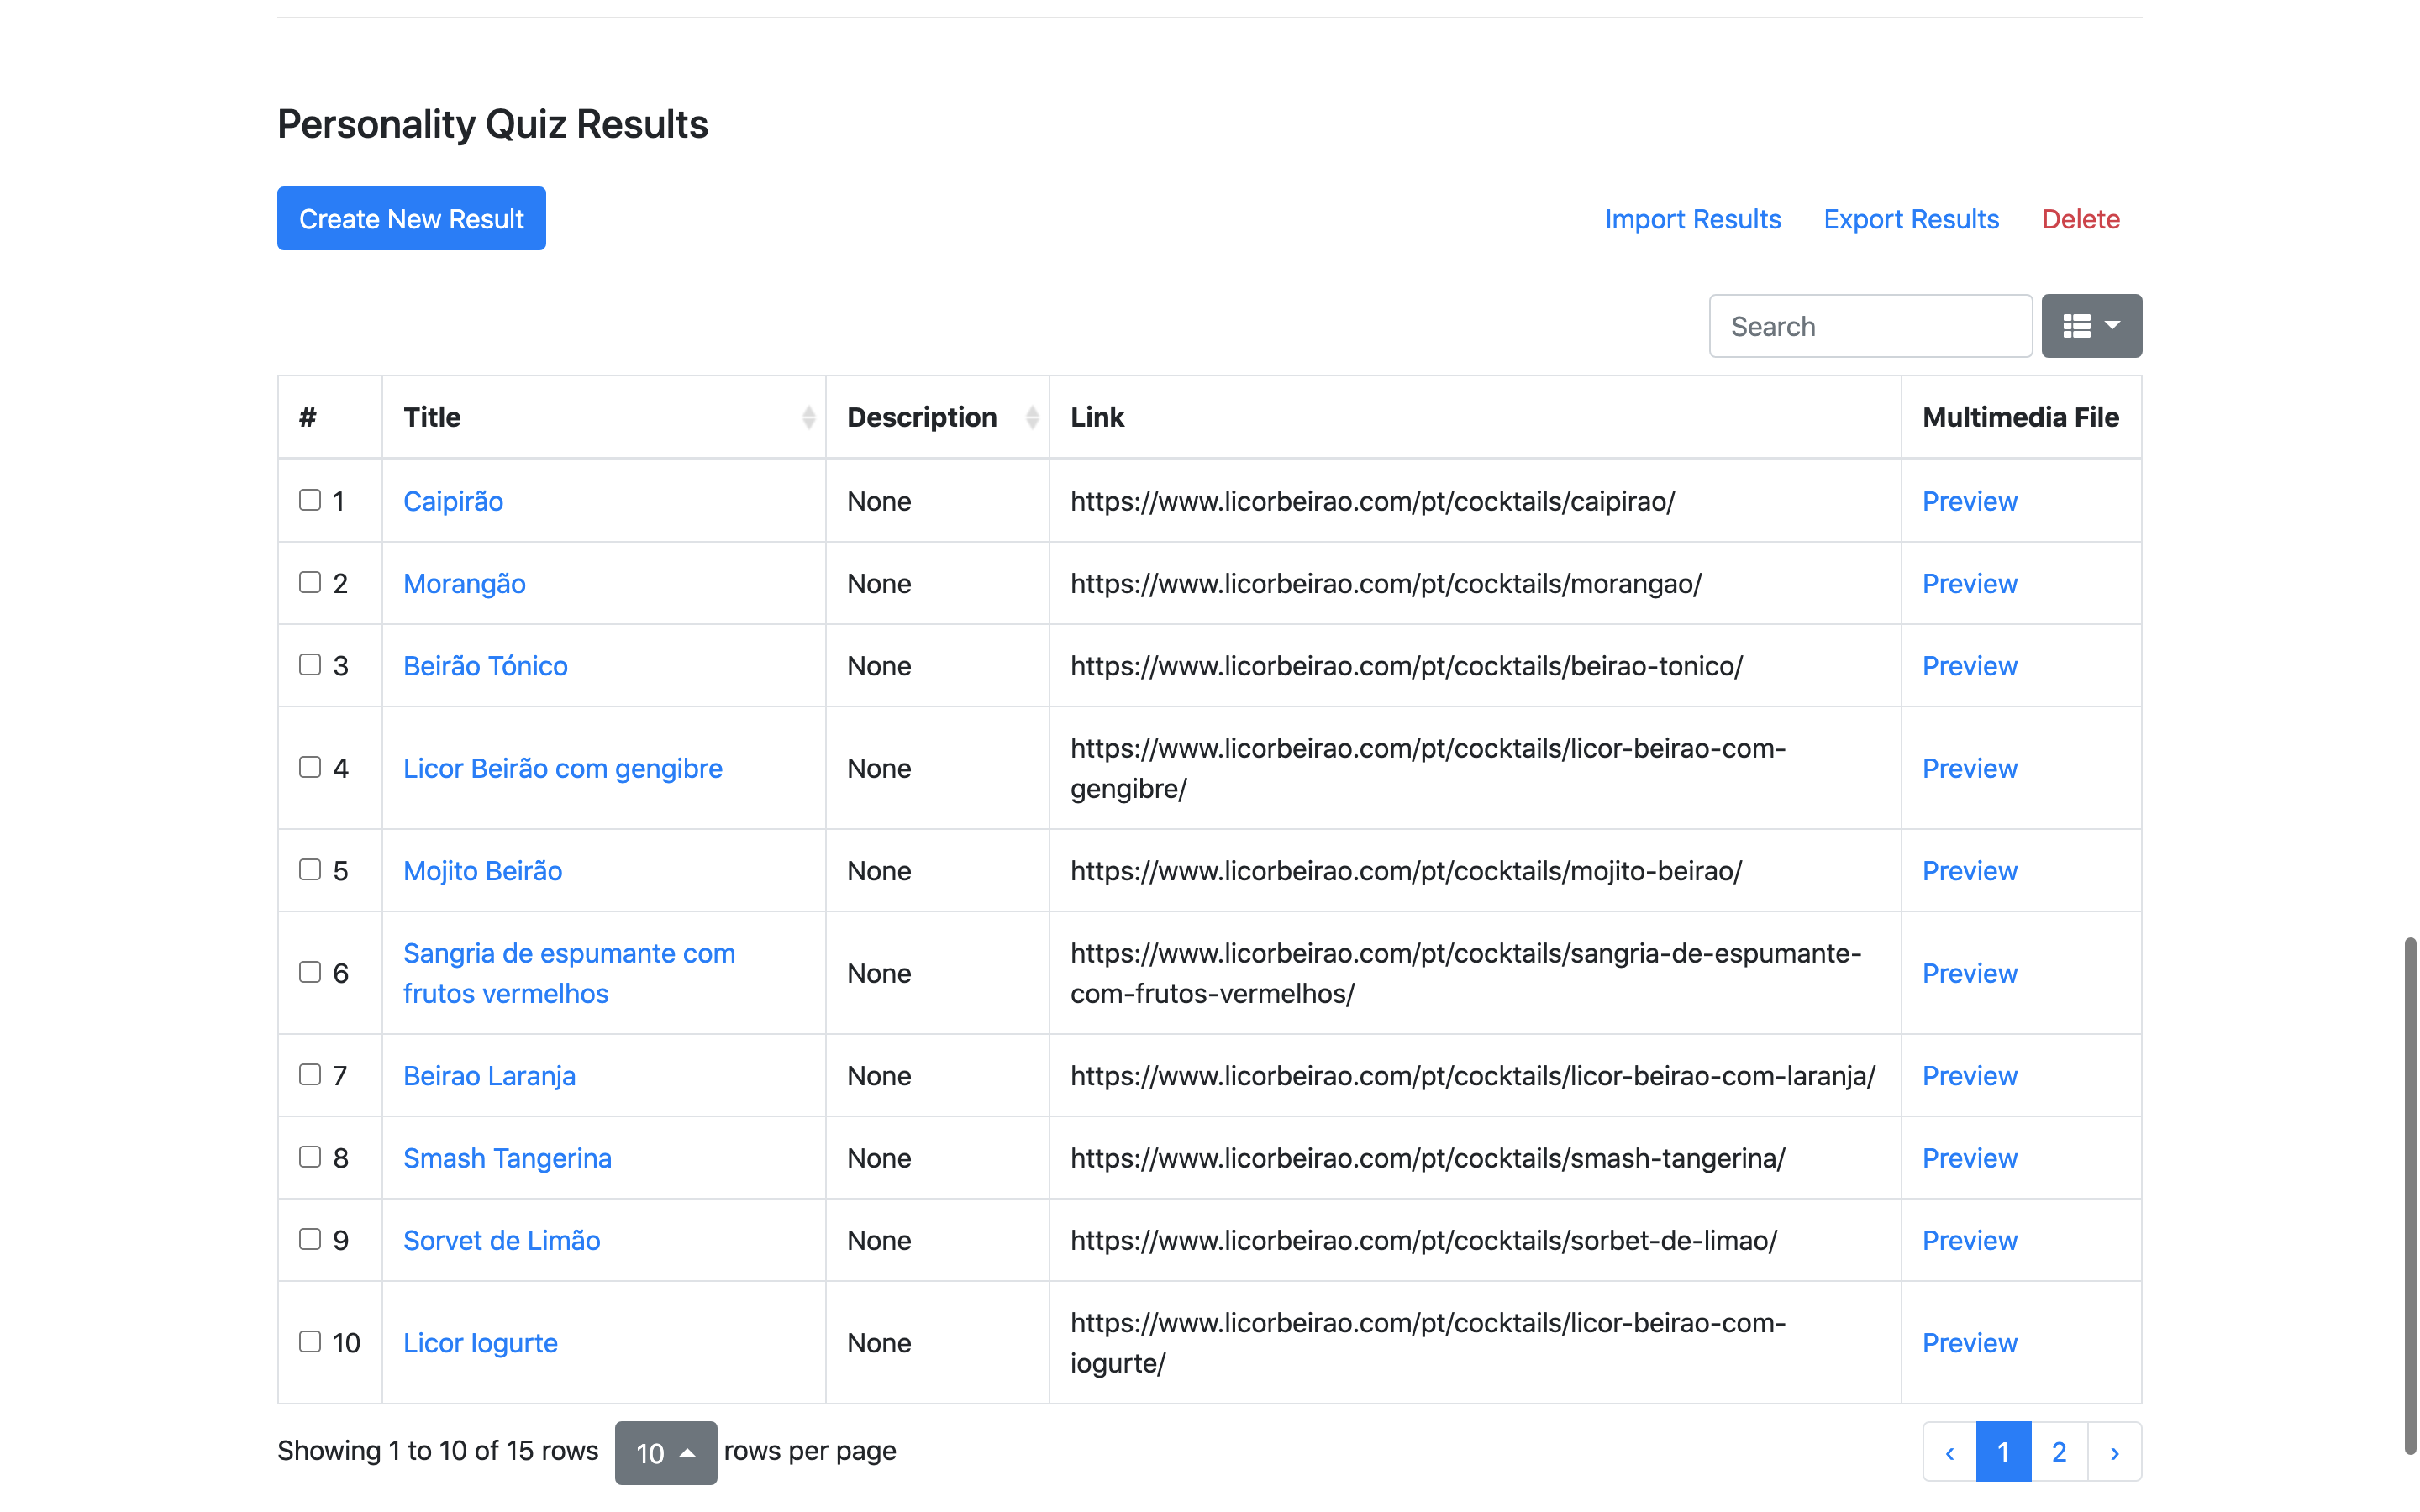
\includegraphics[width=0.8\textwidth]{img/product/pq_results}
		\caption{10.quest - Lista de resultados do Questionário de Personalidade}
		\label{fig:pq_results}
	\end{center}
\end{figure}

\begin{figure}[ht!]
	\begin{center}
		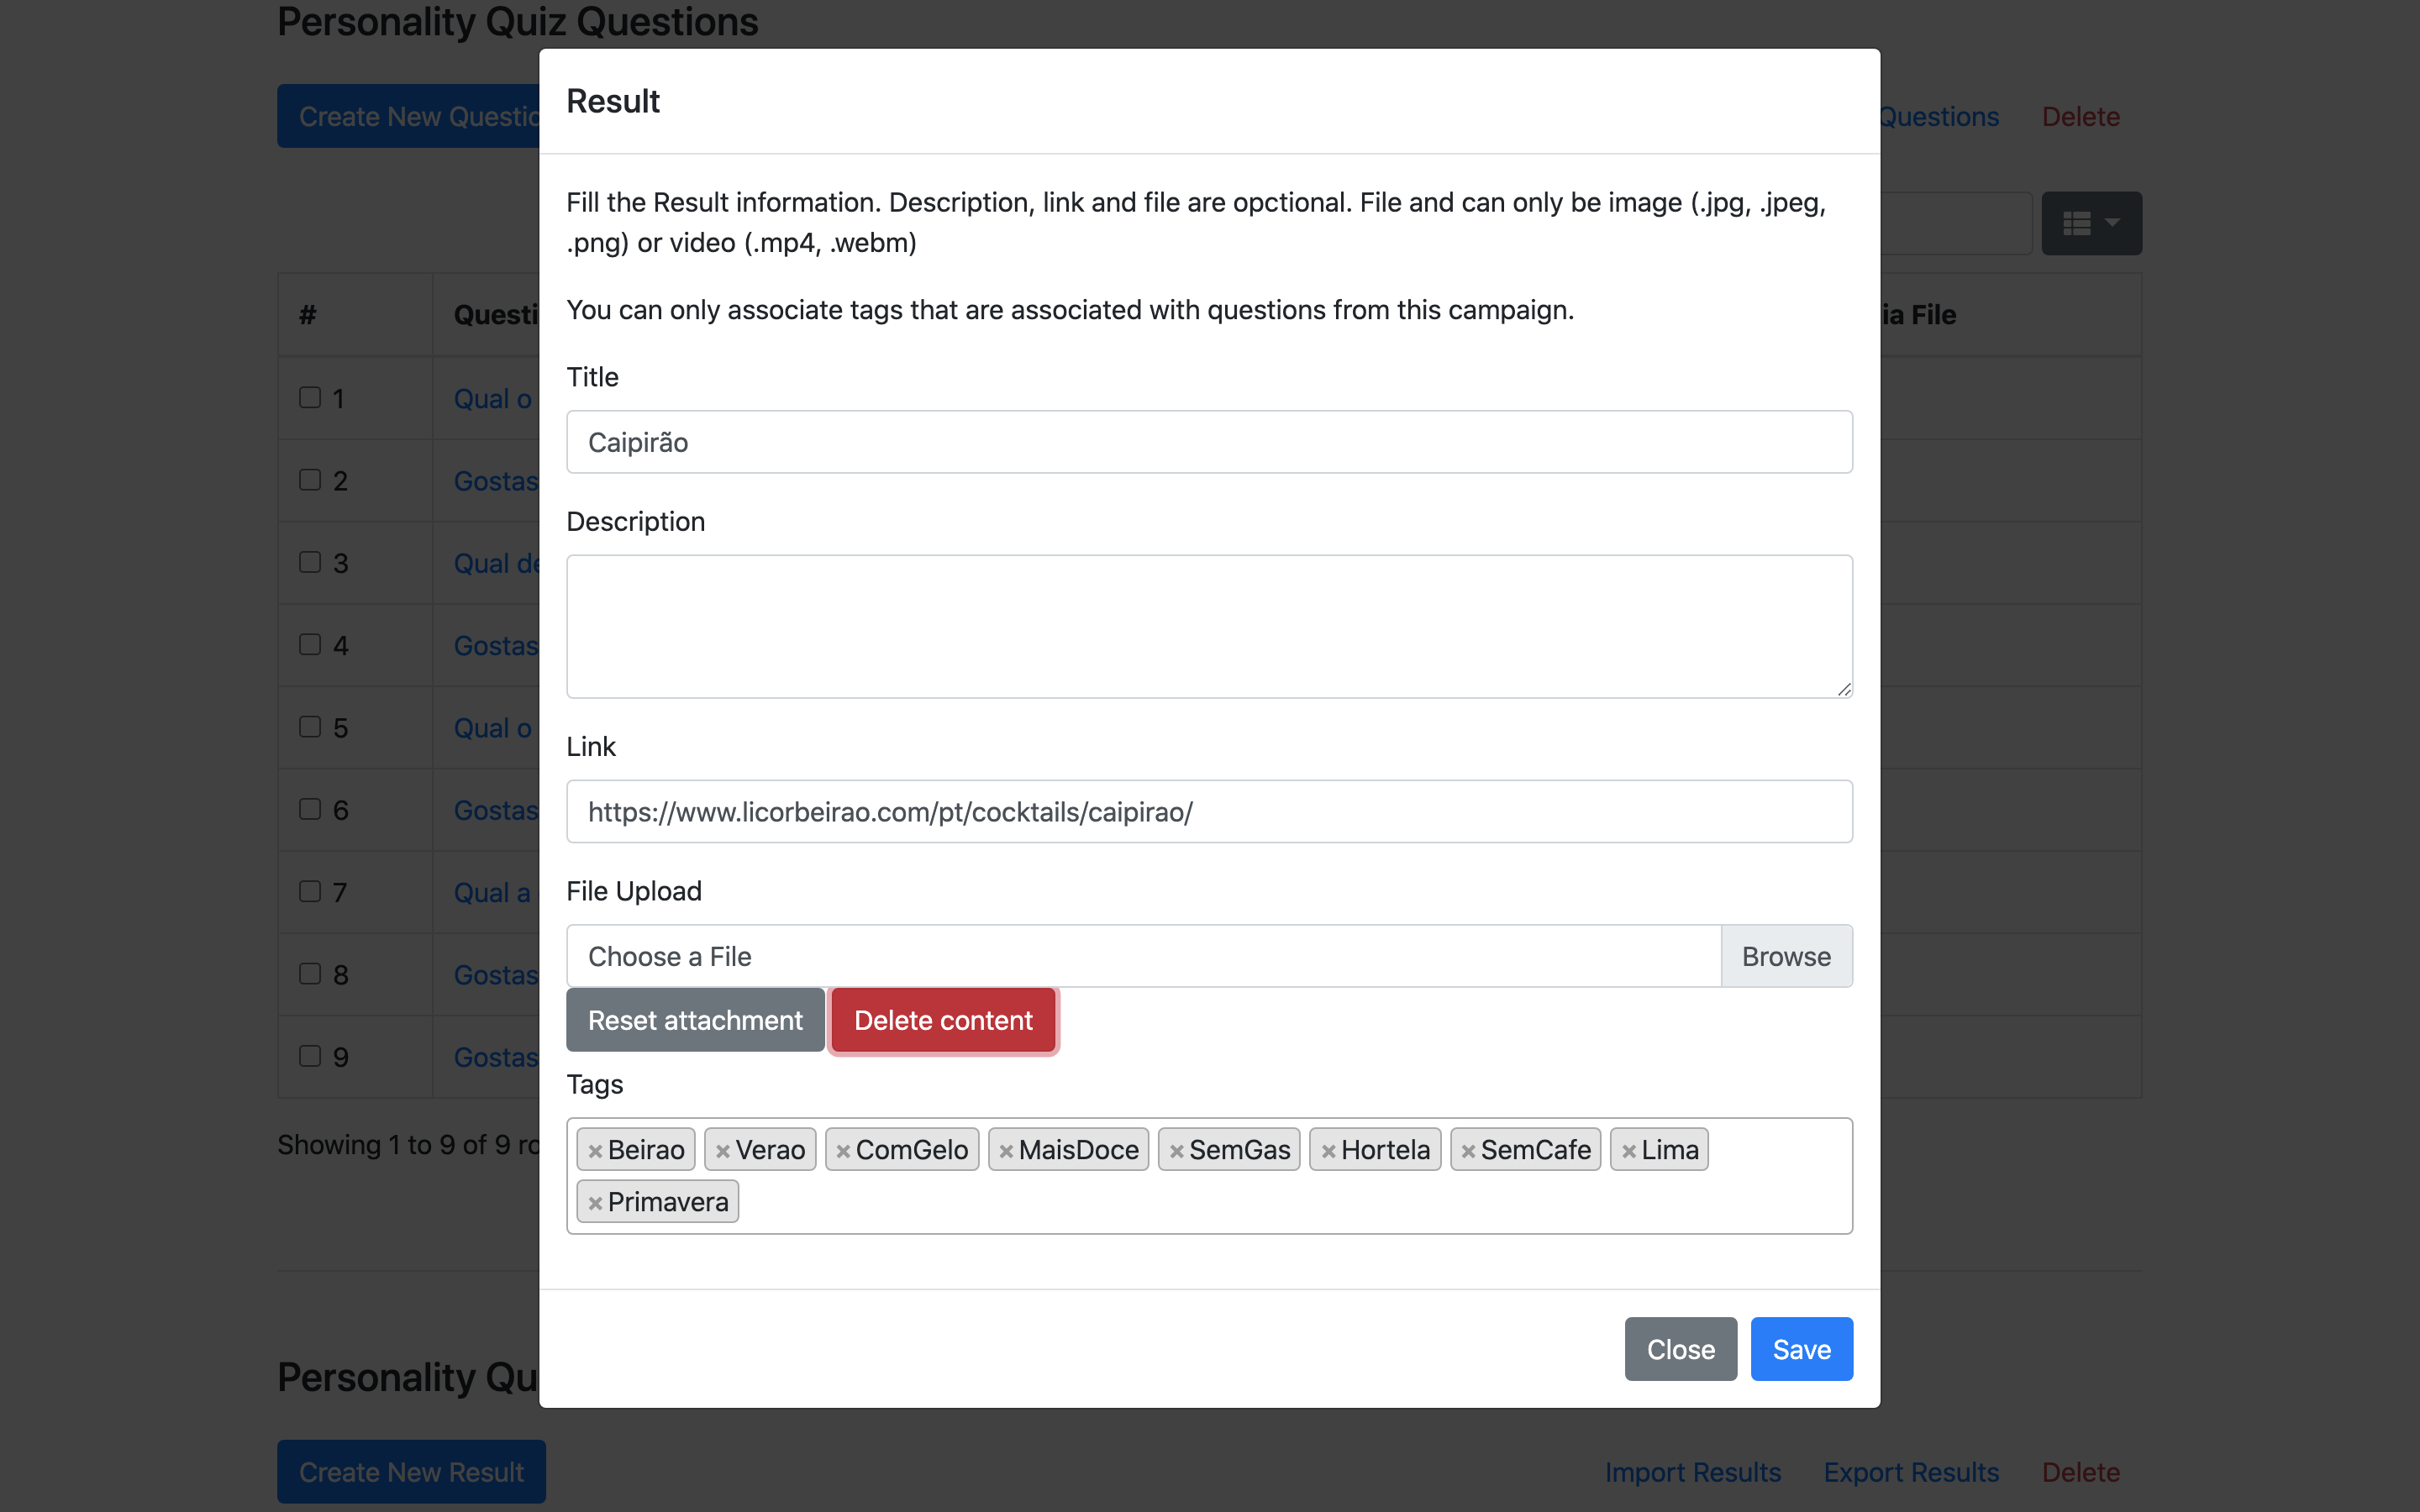
\includegraphics[width=0.8\textwidth]{img/product/pq_result}
		\caption{10.quest - Criar/Editar um resultado}
		\label{fig:pq_result}
	\end{center}
\end{figure}



\section{Trabalho Futuro}

Como foi referido na Capítulo \ref{sec:requisitos}, todas as funcionalidades associadas à criação de campanhas do tipo concurso têm uma prioridade baixa, e neste sentido, será feito um plano futuro para implementar as restantes funcionalidades e cumprir com todos os requisitos funcionais associados ao \textit{back-end} da plataforma.

Tal como referido na secção \ref{sec:dificuldades}, atravessamos atualmente uma situação pandémica e por consequência a empresa ainde se encontra a tentar dar resposta às necessidades do mercado. Foi também referido, que por falta de recursos, o desenvolvimento do \textit{front-end} da plataforma foi minimalista, comparado com o plano inicial, e neste sentido a empresa acredita seriamente que para tirar conclusões de testes de usabilidade é necessário cumprir o desenvolvimento da camada de apresentação (i. e. \textit{front-end}) com o plano original. Assim sendo, assim que a empresa tiver recursos disponíveis, será trabalha a camada de apresentação, juntamente com as funcionalidade referidas no paragrafo anterior.
Durante este período, a plataforma será utilizada como \textit{software beta} pelas empresas do grupo da 10.digital, e desta forma também será possível identificar alguns possíveis ajustes.



%-------------------------------------------------------------------------------------------------
\blankpage
%-------------------------------------------------------------------------------------------------

\glsresetall
